\documentclass[]{article}
\usepackage{lmodern}
\usepackage{amssymb,amsmath}
\usepackage{ifxetex,ifluatex}
\usepackage{fixltx2e} % provides \textsubscript
\ifnum 0\ifxetex 1\fi\ifluatex 1\fi=0 % if pdftex
  \usepackage[T1]{fontenc}
  \usepackage[utf8]{inputenc}
\else % if luatex or xelatex
  \ifxetex
    \usepackage{mathspec}
  \else
    \usepackage{fontspec}
  \fi
  \defaultfontfeatures{Ligatures=TeX,Scale=MatchLowercase}
\fi
% use upquote if available, for straight quotes in verbatim environments
\IfFileExists{upquote.sty}{\usepackage{upquote}}{}
% use microtype if available
\IfFileExists{microtype.sty}{%
\usepackage{microtype}
\UseMicrotypeSet[protrusion]{basicmath} % disable protrusion for tt fonts
}{}
\usepackage[margin=0.6in]{geometry}
\usepackage{hyperref}
\hypersetup{unicode=true,
            pdftitle={MCMC for Bayesian Inference},
            pdfborder={0 0 0},
            breaklinks=true}
\urlstyle{same}  % don't use monospace font for urls
\usepackage{color}
\usepackage{fancyvrb}
\newcommand{\VerbBar}{|}
\newcommand{\VERB}{\Verb[commandchars=\\\{\}]}
\DefineVerbatimEnvironment{Highlighting}{Verbatim}{commandchars=\\\{\}}
% Add ',fontsize=\small' for more characters per line
\usepackage{framed}
\definecolor{shadecolor}{RGB}{248,248,248}
\newenvironment{Shaded}{\begin{snugshade}}{\end{snugshade}}
\newcommand{\KeywordTok}[1]{\textcolor[rgb]{0.13,0.29,0.53}{\textbf{#1}}}
\newcommand{\DataTypeTok}[1]{\textcolor[rgb]{0.13,0.29,0.53}{#1}}
\newcommand{\DecValTok}[1]{\textcolor[rgb]{0.00,0.00,0.81}{#1}}
\newcommand{\BaseNTok}[1]{\textcolor[rgb]{0.00,0.00,0.81}{#1}}
\newcommand{\FloatTok}[1]{\textcolor[rgb]{0.00,0.00,0.81}{#1}}
\newcommand{\ConstantTok}[1]{\textcolor[rgb]{0.00,0.00,0.00}{#1}}
\newcommand{\CharTok}[1]{\textcolor[rgb]{0.31,0.60,0.02}{#1}}
\newcommand{\SpecialCharTok}[1]{\textcolor[rgb]{0.00,0.00,0.00}{#1}}
\newcommand{\StringTok}[1]{\textcolor[rgb]{0.31,0.60,0.02}{#1}}
\newcommand{\VerbatimStringTok}[1]{\textcolor[rgb]{0.31,0.60,0.02}{#1}}
\newcommand{\SpecialStringTok}[1]{\textcolor[rgb]{0.31,0.60,0.02}{#1}}
\newcommand{\ImportTok}[1]{#1}
\newcommand{\CommentTok}[1]{\textcolor[rgb]{0.56,0.35,0.01}{\textit{#1}}}
\newcommand{\DocumentationTok}[1]{\textcolor[rgb]{0.56,0.35,0.01}{\textbf{\textit{#1}}}}
\newcommand{\AnnotationTok}[1]{\textcolor[rgb]{0.56,0.35,0.01}{\textbf{\textit{#1}}}}
\newcommand{\CommentVarTok}[1]{\textcolor[rgb]{0.56,0.35,0.01}{\textbf{\textit{#1}}}}
\newcommand{\OtherTok}[1]{\textcolor[rgb]{0.56,0.35,0.01}{#1}}
\newcommand{\FunctionTok}[1]{\textcolor[rgb]{0.00,0.00,0.00}{#1}}
\newcommand{\VariableTok}[1]{\textcolor[rgb]{0.00,0.00,0.00}{#1}}
\newcommand{\ControlFlowTok}[1]{\textcolor[rgb]{0.13,0.29,0.53}{\textbf{#1}}}
\newcommand{\OperatorTok}[1]{\textcolor[rgb]{0.81,0.36,0.00}{\textbf{#1}}}
\newcommand{\BuiltInTok}[1]{#1}
\newcommand{\ExtensionTok}[1]{#1}
\newcommand{\PreprocessorTok}[1]{\textcolor[rgb]{0.56,0.35,0.01}{\textit{#1}}}
\newcommand{\AttributeTok}[1]{\textcolor[rgb]{0.77,0.63,0.00}{#1}}
\newcommand{\RegionMarkerTok}[1]{#1}
\newcommand{\InformationTok}[1]{\textcolor[rgb]{0.56,0.35,0.01}{\textbf{\textit{#1}}}}
\newcommand{\WarningTok}[1]{\textcolor[rgb]{0.56,0.35,0.01}{\textbf{\textit{#1}}}}
\newcommand{\AlertTok}[1]{\textcolor[rgb]{0.94,0.16,0.16}{#1}}
\newcommand{\ErrorTok}[1]{\textcolor[rgb]{0.64,0.00,0.00}{\textbf{#1}}}
\newcommand{\NormalTok}[1]{#1}
\usepackage{graphicx,grffile}
\makeatletter
\def\maxwidth{\ifdim\Gin@nat@width>\linewidth\linewidth\else\Gin@nat@width\fi}
\def\maxheight{\ifdim\Gin@nat@height>\textheight\textheight\else\Gin@nat@height\fi}
\makeatother
% Scale images if necessary, so that they will not overflow the page
% margins by default, and it is still possible to overwrite the defaults
% using explicit options in \includegraphics[width, height, ...]{}
\setkeys{Gin}{width=\maxwidth,height=\maxheight,keepaspectratio}
\IfFileExists{parskip.sty}{%
\usepackage{parskip}
}{% else
\setlength{\parindent}{0pt}
\setlength{\parskip}{6pt plus 2pt minus 1pt}
}
\setlength{\emergencystretch}{3em}  % prevent overfull lines
\providecommand{\tightlist}{%
  \setlength{\itemsep}{0pt}\setlength{\parskip}{0pt}}
\setcounter{secnumdepth}{0}
% Redefines (sub)paragraphs to behave more like sections
\ifx\paragraph\undefined\else
\let\oldparagraph\paragraph
\renewcommand{\paragraph}[1]{\oldparagraph{#1}\mbox{}}
\fi
\ifx\subparagraph\undefined\else
\let\oldsubparagraph\subparagraph
\renewcommand{\subparagraph}[1]{\oldsubparagraph{#1}\mbox{}}
\fi

%%% Use protect on footnotes to avoid problems with footnotes in titles
\let\rmarkdownfootnote\footnote%
\def\footnote{\protect\rmarkdownfootnote}

%%% Change title format to be more compact
\usepackage{titling}

% Create subtitle command for use in maketitle
\newcommand{\subtitle}[1]{
  \posttitle{
    \begin{center}\large#1\end{center}
    }
}

\setlength{\droptitle}{-2em}

  \title{MCMC for Bayesian Inference}
    \pretitle{\vspace{\droptitle}\centering\huge}
  \posttitle{\par}
    \author{}
    \preauthor{}\postauthor{}
    \date{}
    \predate{}\postdate{}
  
\usepackage{multicol}

\begin{document}
\maketitle

\def\simiid{\stackrel{{\mbox{\text{\tiny i.i.d.}}}}{\sim}}

\subsection{Our Goal}\label{our-goal}

\begin{itemize}
\tightlist
\item
  We want to generate samples from the posterior distribution of a
  parameter \(\theta\) (or possibly a vector of parameters) given the
  observed data.
\end{itemize}

\paragraph{Miscellanea}\label{miscellanea}

MCMC stands for ``Markov chain Monte Carlo''

\begin{itemize}
\tightlist
\item
  Monte Carlo: we will use randomly generated numbers to perform a task
  (estimation of quantities involving the posterior distribution)
\item
  Markov chain: Our numbers will be randomly generated from a Markov
  chain.
\end{itemize}

Notation:

\begin{itemize}
\tightlist
\item
  Denote the pdf of this posterior by \(f(\theta | x_1, \ldots, x_n)\)
\end{itemize}

\subsection{The Metropolis Algorithm}\label{the-metropolis-algorithm}

\begin{multicols}{2}
\begin{enumerate}
\item Pick an initial value, $\theta_1$
\item For $i = 2, 3, \dots, m$:
  \begin{enumerate}
    \item Generate a \textbf{proposal} $\theta_i^*$ for $\theta_i$.
      \begin{itemize}
        \item The proposal is drawn at random from a symmetric distribution that may depend on $\theta_{i-1}$
        \item Example: {\flushleft \hspace{-1cm} $\theta^* | \theta_{i-1} \sim \text{Unif}(\theta_{i-1} - 2, \theta_{i-1} + 2)$}
      \end{itemize}
    \item Calculate the \textbf{acceptance probability} {\flushleft \hspace{-2.5cm} $r = \begin{cases} \frac{f(\theta^*|x_1, \ldots, x_n)}{f(\theta_{i-1} | x_1, \ldots, x_n)} \text{ if $f(\theta^*|x_1, \ldots, x_n) \leq f(\theta_{i-1} | x_1, \ldots, x_n)$} \\ 1 \text{ if $f(\theta^*|x_1, \ldots, x_n) > f(\theta_{i-1} | x_1, \ldots, x_n)$} \end{cases}$}
    \item Set $\theta_i = \begin{cases} \theta^* \text{ with probability $r$} \\ \theta_{i-1} \text{ with probability $1-r$} \end{cases}$
  \end{enumerate}
\end{enumerate}
$\hphantom{5}$ \\
$\hphantom{5}$ \\
$\hphantom{5}$ \\
$\hphantom{5}$ \\
$\hphantom{5}$ \\
$\hphantom{5}$ \\
$\hphantom{5}$ \\
$\hphantom{5}$ \\
$\hphantom{5}$ \\
$\hphantom{5}$ \\
$\hphantom{5}$ \\
$\hphantom{5}$ \\
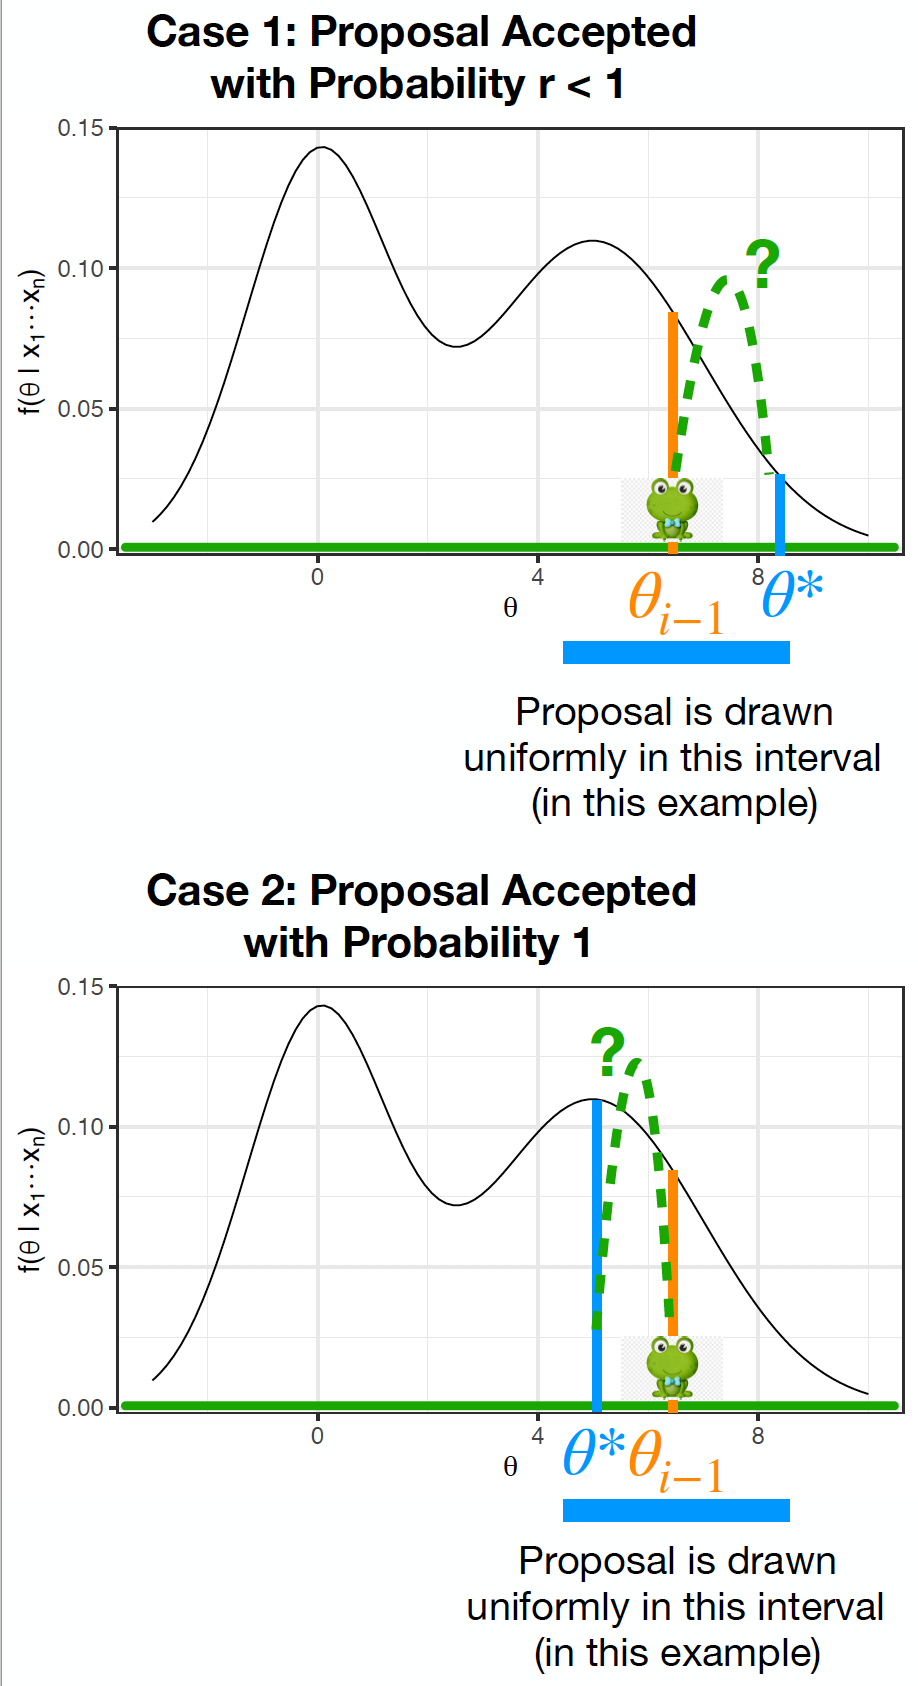
\includegraphics[width=3.3in]{mcmc_illustration.png}
\end{multicols}

\newpage

\textbf{Definition:} A Markov chain is a sequence of random variables
\(X_1, X_2, \ldots\) with the property that for any set \(A\),

\(P(X_i \in A | X_1 = x_1, X_2 = x_2, \ldots, X_{i-1} = x_{i-1}) = P(X_i \in A | X_{i-1} = x_{i-1})\)

\begin{itemize}
\tightlist
\item
  Intuition: the distribution of \(X_i\) depends only on \(X_{i-1}\)
\end{itemize}

\textbf{Example:} The sequence of random variables
\(\Theta_1, \Theta_2, \ldots\) from the Metropolis algorithm form a
Markov chain

\textbf{Remarkable fact 1:} If some conditions are satisfied then the
distribution of \(X_i\) converges to a given \textbf{stationary
distribution} as \(i \rightarrow \infty\).

\begin{itemize}
\tightlist
\item
  The stationary distribution depends on the transition distribution for
  moving from \(X_{i-1}\) to \(X_i\).
\item
  The stationary distribution does not depend on your choice of \(X_1\)!
\end{itemize}

For proofs of things like this, see Math 339SP: Stochastic Processes.

\textbf{Remarkable fact 2:} For the Metropolis algorithm above, the
stationary distribution is the posterior distribution for \(\Theta\).

In practice, the sampler can take a while to converge to the stationary
distribution. We typically throw away the first several hundred samples
as \emph{burn-in}.

To check for convergence, we can run multiple chains that started from
different random starting points and compare the results; if the samples
from all four chains look similar, that's evidence that they have
converged.

\subsubsection{Example: Cosmological Microwave Background
(CMB)}\label{example-cosmological-microwave-background-cmb}

This example is taken from Marin and Robert (2007). Here's a quote from
them describing the figure below, also from them:

\begin{quote}
'Figure 2.2 is an image (in the spectral domain) of the ``cosmological
microwave background'' (CMB) in a region of the sky: More specifically,
this picture represents the electromagnetic radiation from photons
dating back to the early ages of the universe, a radiation often called
``fossil light,'' that dates back to a few hundred thousand years after
the Big Bang (Chown, 1996). The grey levels are given by the differences
in apparent temperature from the mean temperature and as stored in
\texttt{cmb}.
\end{quote}

\begin{quote}
For astrophysical (or rather cosmological) reasons too involved to be
detailed here, the repartition of the sectrum is quite isotropic (that
is, independent of direction) and normal. In fact, if we treat each
temperature difference in Figure 2.2 as an independent realization, the
histogram of these differences \ldots{} provides a rather accurate
representation of the distribution of these temperatures\ldots{}'
\end{quote}

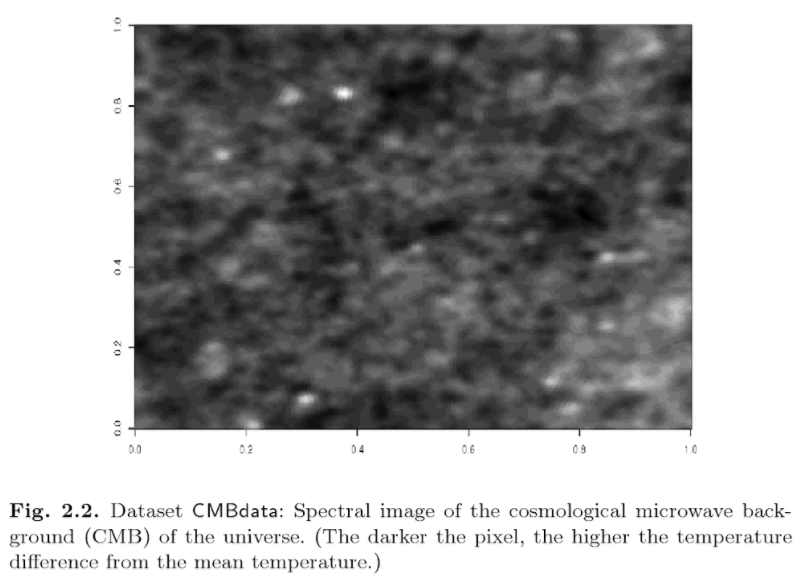
\includegraphics[height = 4in]{CMBdata_bayesian_core.png}

The code below reads in the data and makes an initial plot:

\begin{Shaded}
\begin{Highlighting}[]
\KeywordTok{library}\NormalTok{(tidyverse)}

\NormalTok{cmb <-}\StringTok{ }\KeywordTok{read_csv}\NormalTok{(}\StringTok{"http://www.evanlray.com/data/bayesian_core/CMBdata.txt"}\NormalTok{,}
    \DataTypeTok{col_names =} \OtherTok{FALSE}\NormalTok{)}
\KeywordTok{names}\NormalTok{(cmb) <-}\StringTok{ "temp_difference"}

\KeywordTok{ggplot}\NormalTok{(}\DataTypeTok{data =}\NormalTok{ cmb, }\DataTypeTok{mapping =} \KeywordTok{aes}\NormalTok{(}\DataTypeTok{x =}\NormalTok{ temp_difference)) }\OperatorTok{+}
\StringTok{  }\KeywordTok{geom_histogram}\NormalTok{(}\DataTypeTok{center =} \FloatTok{0.005}\NormalTok{, }\DataTypeTok{binwidth =} \FloatTok{0.01}\NormalTok{, }\DataTypeTok{mapping =} \KeywordTok{aes}\NormalTok{(}\DataTypeTok{y =}\NormalTok{ ..density..))}
\end{Highlighting}
\end{Shaded}

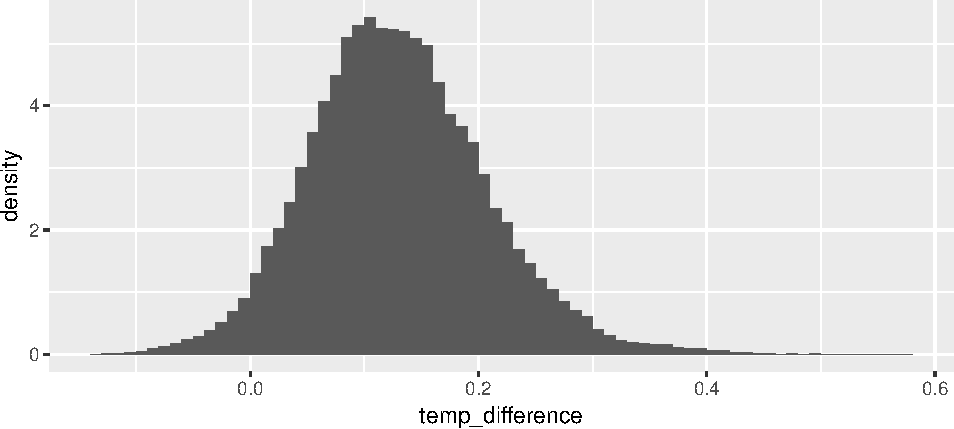
\includegraphics{20190225_bayes_MCMC_Metropolis_files/figure-latex/unnamed-chunk-1-1.pdf}

\paragraph{Model}\label{model}

It appears that a normal model would be reasonable for these data. To be
formal, let \(X_1, \ldots, X_n\) denote the \(n = 640000\) temperature
differences. We model these as independent, with each

\(X_i \sim \text{Normal}(\mu, \sigma^2)\)

This model has two parameters: \(\mu\) and \(\sigma^2\). We will use the
following prior distributions for these parameters:

An improper, non-informative prior for \(\mu\):

\(f(\mu) = 1\)

A Gamma\((2, 1)\) prior for \(\sigma^2\):

\(f(\sigma^2 | \alpha = 2, \beta = 1) = \frac{\beta^\alpha}{\Gamma(\alpha)}(\sigma^2)^{\alpha - 1}e^{-\beta x}\)

The probability density function of the posterior distribution for
\(\mu\) and \(\sigma^2\) is therefore equal to a constant \(c\) times
the prior pdfs times the data model pdf:

\begin{align*}
f(\mu, \sigma^2 | \alpha = 2, \beta = 1, x_1, \ldots, x_n) &= c \cdot f(\mu) \cdot f(\sigma^2 | \alpha = 2, \beta = 1) \cdot f(x_1, \ldots, x_n | \mu, \sigma^2) \\
&= c \cdot 1 \cdot \frac{\beta^\alpha}{\Gamma(\alpha)}(\sigma^2)^{\alpha - 1}e^{-\beta x} \cdot \prod_{i=1}^n \frac{1}{\sqrt{2 \pi \sigma^2}} \exp\left[ \frac{-1}{2 \sigma^2} (x_i - \mu)^2 \right]
\end{align*}

The posterior distribution is involved. Rather than trying to understand
it analytically, let's take a sample from the joint posterior
distribution of \(\mu\) and \(\sigma^2\), and use that to examine the
posterior distribution.

\section{Samples from the posterior
distribution}\label{samples-from-the-posterior-distribution}

\begin{Shaded}
\begin{Highlighting}[]
\CommentTok{# how many samples to draw from the posterior}
\NormalTok{sample_size <-}\StringTok{ }\DecValTok{10000}

\CommentTok{# How many to throw away?  (Assuming convergence after this)}
\NormalTok{burn_in <-}\StringTok{ }\DecValTok{100}

\CommentTok{# allocate data frame to store results}
\NormalTok{theta_posterior_sample <-}\StringTok{ }\KeywordTok{data.frame}\NormalTok{(}
  \DataTypeTok{mu =} \KeywordTok{rep}\NormalTok{(}\OtherTok{NA}\NormalTok{, sample_size }\OperatorTok{+}\StringTok{ }\NormalTok{burn_in),}
  \DataTypeTok{log_sigma_sq =} \KeywordTok{rep}\NormalTok{(}\OtherTok{NA}\NormalTok{, sample_size }\OperatorTok{+}\StringTok{ }\NormalTok{burn_in),}
  \DataTypeTok{sigma_sq =} \KeywordTok{rep}\NormalTok{(}\OtherTok{NA}\NormalTok{, sample_size }\OperatorTok{+}\StringTok{ }\NormalTok{burn_in)}
\NormalTok{)}

\CommentTok{# set initial values/first sample/Markov chain starting point}
\NormalTok{theta_posterior_sample}\OperatorTok{$}\NormalTok{mu[}\DecValTok{1}\NormalTok{] <-}\StringTok{ }\KeywordTok{mean}\NormalTok{(cmb}\OperatorTok{$}\NormalTok{temp_difference)}
\NormalTok{theta_posterior_sample}\OperatorTok{$}\NormalTok{log_sigma_sq[}\DecValTok{1}\NormalTok{] <-}\StringTok{ }\KeywordTok{log}\NormalTok{(}\KeywordTok{var}\NormalTok{(cmb}\OperatorTok{$}\NormalTok{temp_difference))}
\NormalTok{theta_posterior_sample}\OperatorTok{$}\NormalTok{sigma_sq[}\DecValTok{1}\NormalTok{] <-}\StringTok{ }\KeywordTok{var}\NormalTok{(cmb}\OperatorTok{$}\NormalTok{temp_difference)}

\CommentTok{# Sequentially, obtain the remaining samples}
\ControlFlowTok{for}\NormalTok{(i }\ControlFlowTok{in} \KeywordTok{seq}\NormalTok{(}\DataTypeTok{from =} \DecValTok{2}\NormalTok{, }\DataTypeTok{to =}\NormalTok{ sample_size }\OperatorTok{+}\StringTok{ }\NormalTok{burn_in)) \{}
    \CommentTok{# Generate a proposal for the next value of theta, from a}
    \CommentTok{# Uniform(previous_theta - 0.1, previous_theta + 0.1) distribution}
\NormalTok{    previous_mu <-}\StringTok{ }\NormalTok{theta_posterior_sample}\OperatorTok{$}\NormalTok{mu[i}\OperatorTok{-}\DecValTok{1}\NormalTok{]}
\NormalTok{    previous_log_sigma_sq <-}\StringTok{ }\NormalTok{theta_posterior_sample}\OperatorTok{$}\NormalTok{log_sigma_sq[i}\OperatorTok{-}\DecValTok{1}\NormalTok{]}
\NormalTok{    mu_proposal <-}\StringTok{ }\KeywordTok{runif}\NormalTok{(}\DecValTok{1}\NormalTok{, previous_mu }\OperatorTok{-}\StringTok{ }\NormalTok{.}\DecValTok{001}\NormalTok{, previous_mu }\OperatorTok{+}\StringTok{ }\NormalTok{.}\DecValTok{001}\NormalTok{)}
\NormalTok{    log_sigma_sq_proposal <-}\StringTok{ }\KeywordTok{runif}\NormalTok{(}\DecValTok{1}\NormalTok{, previous_log_sigma_sq }\OperatorTok{-}\StringTok{ }\NormalTok{.}\DecValTok{001}\NormalTok{, previous_log_sigma_sq }\OperatorTok{+}\StringTok{ }\NormalTok{.}\DecValTok{001}\NormalTok{)}
    
    \CommentTok{# calculate probability of accepting the proposal}
\NormalTok{    log_r_num <-}\StringTok{ }\KeywordTok{dgamma}\NormalTok{(}\KeywordTok{exp}\NormalTok{(log_sigma_sq_proposal), }\DataTypeTok{shape =} \DecValTok{2}\NormalTok{, }\DataTypeTok{rate =} \DecValTok{1}\NormalTok{, }\DataTypeTok{log =} \OtherTok{TRUE}\NormalTok{) }\OperatorTok{+}
\StringTok{        }\KeywordTok{sum}\NormalTok{(}\KeywordTok{dnorm}\NormalTok{(cmb}\OperatorTok{$}\NormalTok{temp_difference,}
                  \DataTypeTok{mean =}\NormalTok{ mu_proposal,}
                  \DataTypeTok{sd =} \KeywordTok{sqrt}\NormalTok{(}\KeywordTok{exp}\NormalTok{(log_sigma_sq_proposal)),}
                  \DataTypeTok{log =} \OtherTok{TRUE}\NormalTok{))}
\NormalTok{    log_r_denom <-}\StringTok{ }\KeywordTok{dgamma}\NormalTok{(}\KeywordTok{exp}\NormalTok{(previous_log_sigma_sq), }\DataTypeTok{shape =} \DecValTok{2}\NormalTok{, }\DataTypeTok{rate =} \DecValTok{1}\NormalTok{, }\DataTypeTok{log =} \OtherTok{TRUE}\NormalTok{) }\OperatorTok{+}
\StringTok{        }\KeywordTok{sum}\NormalTok{(}\KeywordTok{dnorm}\NormalTok{(cmb}\OperatorTok{$}\NormalTok{temp_difference,}
                  \DataTypeTok{mean =}\NormalTok{ previous_mu,}
                  \DataTypeTok{sd =} \KeywordTok{sqrt}\NormalTok{(}\KeywordTok{exp}\NormalTok{(previous_log_sigma_sq)),}
                  \DataTypeTok{log =} \OtherTok{TRUE}\NormalTok{))}
    
    \CommentTok{# calculate acceptance probability}
    \ControlFlowTok{if}\NormalTok{(log_r_num }\OperatorTok{>}\StringTok{ }\NormalTok{log_r_denom) \{}
\NormalTok{      r <-}\StringTok{ }\DecValTok{1}
\NormalTok{    \} }\ControlFlowTok{else}\NormalTok{ \{}
\NormalTok{      r <-}\StringTok{ }\KeywordTok{exp}\NormalTok{(log_r_num }\OperatorTok{-}\StringTok{ }\NormalTok{log_r_denom)}
\NormalTok{    \}}
    
    \CommentTok{# accept the proposal or not, with the appropriate probability}
    \ControlFlowTok{if}\NormalTok{(}\KeywordTok{rbinom}\NormalTok{(}\DecValTok{1}\NormalTok{, }\DecValTok{1}\NormalTok{, r) }\OperatorTok{==}\StringTok{ }\DecValTok{1}\NormalTok{) \{}
\NormalTok{        theta_posterior_sample}\OperatorTok{$}\NormalTok{mu[i] <-}\StringTok{ }\NormalTok{mu_proposal}
\NormalTok{        theta_posterior_sample}\OperatorTok{$}\NormalTok{log_sigma_sq[i] <-}\StringTok{ }\NormalTok{log_sigma_sq_proposal}
\NormalTok{        theta_posterior_sample}\OperatorTok{$}\NormalTok{sigma_sq[i] <-}\StringTok{ }\KeywordTok{exp}\NormalTok{(log_sigma_sq_proposal)}
\NormalTok{    \} }\ControlFlowTok{else}\NormalTok{ \{}
\NormalTok{        theta_posterior_sample}\OperatorTok{$}\NormalTok{mu[i] <-}\StringTok{ }\NormalTok{previous_mu}
\NormalTok{        theta_posterior_sample}\OperatorTok{$}\NormalTok{log_sigma_sq[i] <-}\StringTok{ }\NormalTok{previous_log_sigma_sq}
\NormalTok{        theta_posterior_sample}\OperatorTok{$}\NormalTok{sigma_sq[i] <-}\StringTok{ }\KeywordTok{exp}\NormalTok{(previous_log_sigma_sq)}
\NormalTok{    \}}
\NormalTok{\}}

\CommentTok{# discard burn-in}
\NormalTok{theta_posterior_sample <-}\StringTok{ }\NormalTok{theta_posterior_sample[}\OperatorTok{-}\KeywordTok{seq_len}\NormalTok{(burn_in), ]}
\end{Highlighting}
\end{Shaded}

\begin{Shaded}
\begin{Highlighting}[]
\KeywordTok{head}\NormalTok{(theta_posterior_sample)}
\end{Highlighting}
\end{Shaded}

\begin{verbatim}
##            mu log_sigma_sq    sigma_sq
## 101 0.1296762    -5.116966 0.005994183
## 102 0.1296762    -5.116966 0.005994183
## 103 0.1296762    -5.116966 0.005994183
## 104 0.1296762    -5.116966 0.005994183
## 105 0.1296762    -5.116966 0.005994183
## 106 0.1296762    -5.116966 0.005994183
\end{verbatim}

\paragraph{\texorpdfstring{Plots to represent the approximate joint
posterior distribution of
\(\mu, \sigma^2\)}{Plots to represent the approximate joint posterior distribution of \textbackslash{}mu, \textbackslash{}sigma\^{}2}}\label{plots-to-represent-the-approximate-joint-posterior-distribution-of-mu-sigma2}

Each point in the plot is a sample from the joint posterior of
\(\mu, \sigma^2 | x_1, \ldots, x_n\).

\begin{Shaded}
\begin{Highlighting}[]
\KeywordTok{ggplot}\NormalTok{(}\DataTypeTok{data =}\NormalTok{ theta_posterior_sample, }\DataTypeTok{mapping =} \KeywordTok{aes}\NormalTok{(}\DataTypeTok{x =}\NormalTok{ mu, }\DataTypeTok{y =}\NormalTok{ sigma_sq)) }\OperatorTok{+}
\StringTok{  }\KeywordTok{geom_point}\NormalTok{(}\DataTypeTok{alpha =} \FloatTok{0.4}\NormalTok{)}
\end{Highlighting}
\end{Shaded}

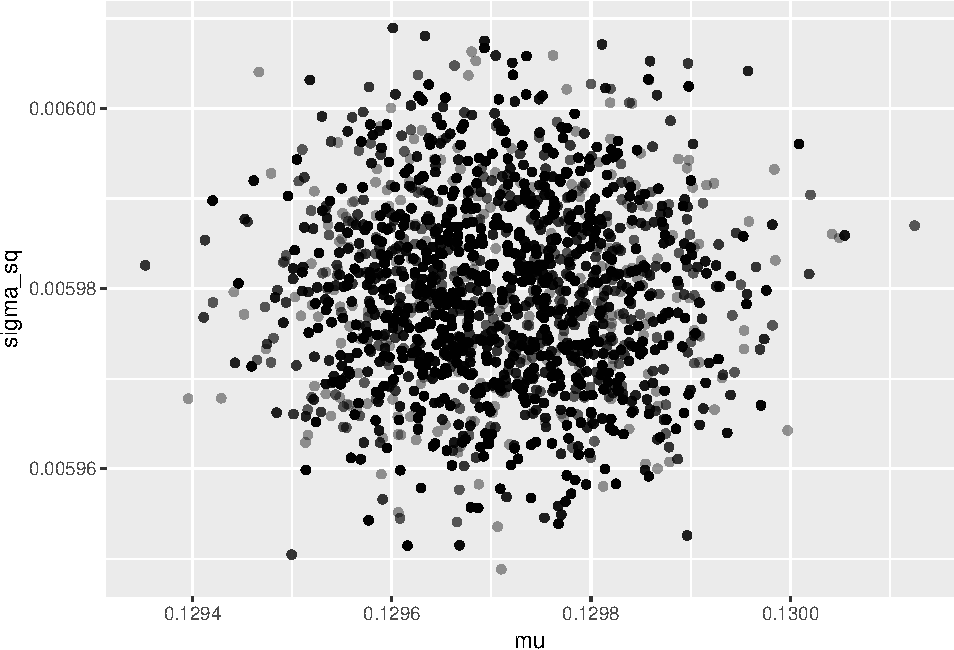
\includegraphics{20190225_bayes_MCMC_Metropolis_files/figure-latex/unnamed-chunk-5-1.pdf}

\begin{Shaded}
\begin{Highlighting}[]
\KeywordTok{ggplot}\NormalTok{(}\DataTypeTok{data =}\NormalTok{ theta_posterior_sample, }\DataTypeTok{mapping =} \KeywordTok{aes}\NormalTok{(}\DataTypeTok{x =}\NormalTok{ mu, }\DataTypeTok{y =}\NormalTok{ sigma_sq)) }\OperatorTok{+}
\StringTok{  }\KeywordTok{geom_density2d}\NormalTok{()}
\end{Highlighting}
\end{Shaded}

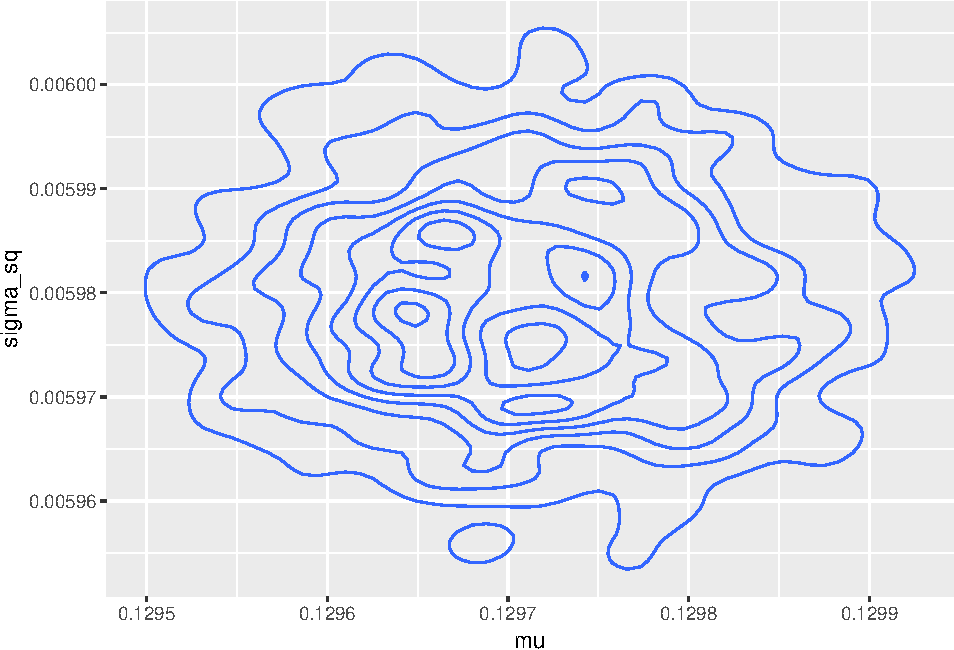
\includegraphics{20190225_bayes_MCMC_Metropolis_files/figure-latex/unnamed-chunk-6-1.pdf}

\begin{Shaded}
\begin{Highlighting}[]
\KeywordTok{ggplot}\NormalTok{(}\DataTypeTok{data =}\NormalTok{ theta_posterior_sample, }\DataTypeTok{mapping =} \KeywordTok{aes}\NormalTok{(}\DataTypeTok{x =}\NormalTok{ mu, }\DataTypeTok{y =}\NormalTok{ sigma_sq)) }\OperatorTok{+}
\StringTok{  }\KeywordTok{geom_density2d}\NormalTok{(}\DataTypeTok{h =} \KeywordTok{c}\NormalTok{(}\FloatTok{0.00015}\NormalTok{, }\FloatTok{0.000015}\NormalTok{))}
\end{Highlighting}
\end{Shaded}

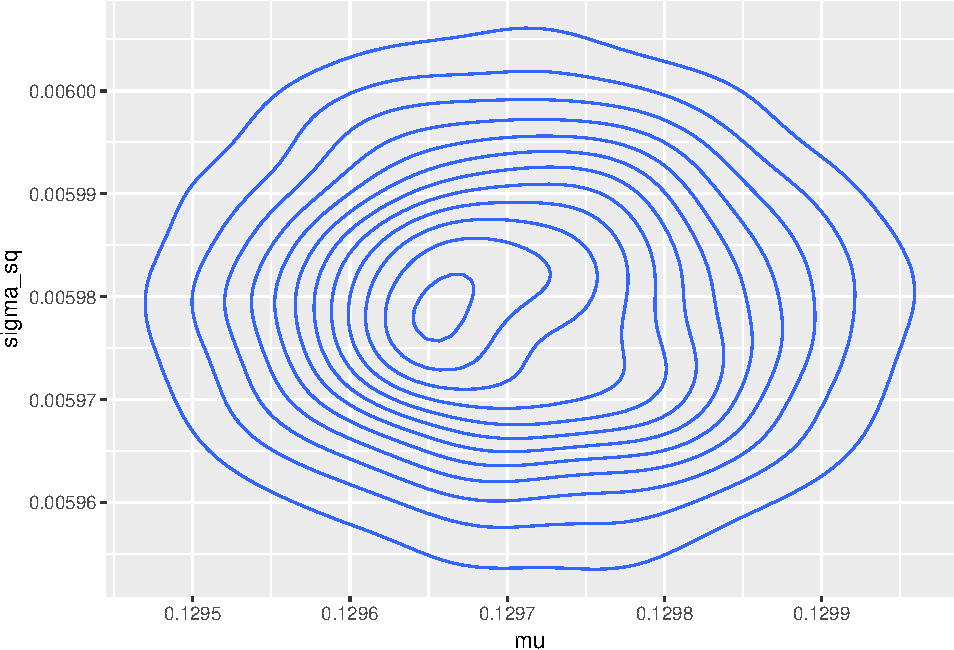
\includegraphics{20190225_bayes_MCMC_Metropolis_files/figure-latex/unnamed-chunk-7-1.pdf}

\newpage

\paragraph{\texorpdfstring{Plots to represent the approximate marginal
posterior distribution of
\(\mu\)}{Plots to represent the approximate marginal posterior distribution of \textbackslash{}mu}}\label{plots-to-represent-the-approximate-marginal-posterior-distribution-of-mu}

\begin{Shaded}
\begin{Highlighting}[]
\KeywordTok{ggplot}\NormalTok{() }\OperatorTok{+}
\StringTok{  }\KeywordTok{geom_histogram}\NormalTok{(}\DataTypeTok{data =}\NormalTok{ theta_posterior_sample, }\DataTypeTok{mapping =} \KeywordTok{aes}\NormalTok{(}\DataTypeTok{x =}\NormalTok{ mu, }\DataTypeTok{y =}\NormalTok{ ..density..))}
\end{Highlighting}
\end{Shaded}

\begin{verbatim}
## `stat_bin()` using `bins = 30`. Pick better value with `binwidth`.
\end{verbatim}

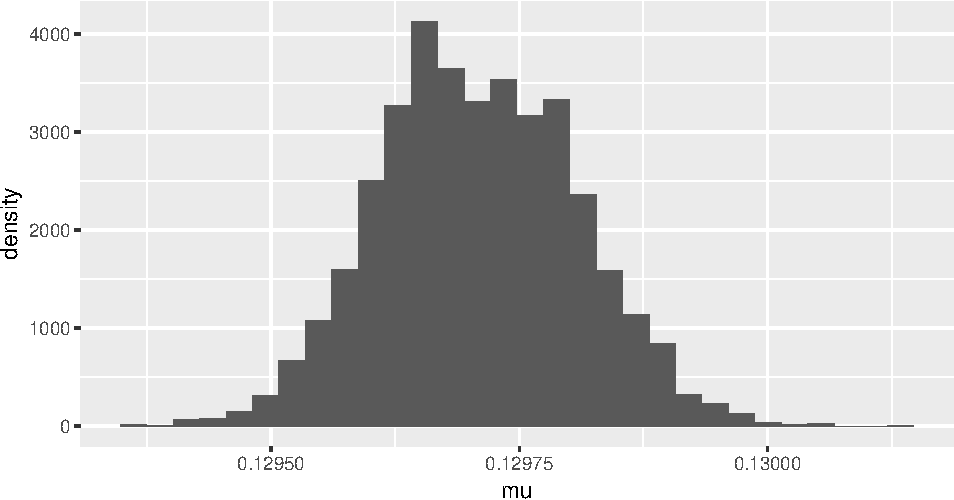
\includegraphics{20190225_bayes_MCMC_Metropolis_files/figure-latex/unnamed-chunk-8-1.pdf}

\begin{Shaded}
\begin{Highlighting}[]
\KeywordTok{ggplot}\NormalTok{() }\OperatorTok{+}
\StringTok{  }\KeywordTok{geom_density}\NormalTok{(}\DataTypeTok{data =}\NormalTok{ theta_posterior_sample, }\DataTypeTok{mapping =} \KeywordTok{aes}\NormalTok{(}\DataTypeTok{x =}\NormalTok{ mu))}
\end{Highlighting}
\end{Shaded}

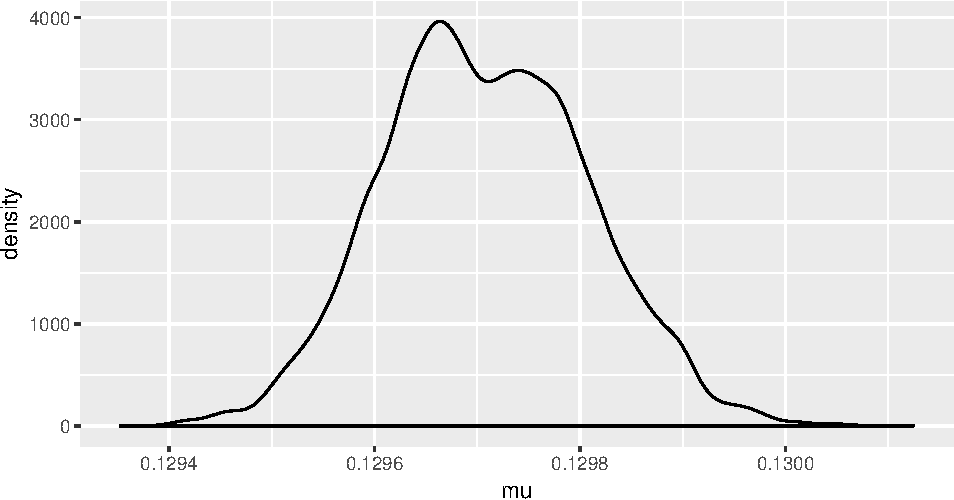
\includegraphics{20190225_bayes_MCMC_Metropolis_files/figure-latex/unnamed-chunk-9-1.pdf}

\newpage

\paragraph{\texorpdfstring{Plots to represent the approximate marginal
posterior distribution of
\(\sigma^2\)}{Plots to represent the approximate marginal posterior distribution of \textbackslash{}sigma\^{}2}}\label{plots-to-represent-the-approximate-marginal-posterior-distribution-of-sigma2}

\begin{Shaded}
\begin{Highlighting}[]
\KeywordTok{ggplot}\NormalTok{() }\OperatorTok{+}
\StringTok{  }\KeywordTok{geom_histogram}\NormalTok{(}\DataTypeTok{data =}\NormalTok{ theta_posterior_sample, }\DataTypeTok{mapping =} \KeywordTok{aes}\NormalTok{(}\DataTypeTok{x =}\NormalTok{ sigma_sq, }\DataTypeTok{y =}\NormalTok{ ..density..))}
\end{Highlighting}
\end{Shaded}

\begin{verbatim}
## `stat_bin()` using `bins = 30`. Pick better value with `binwidth`.
\end{verbatim}

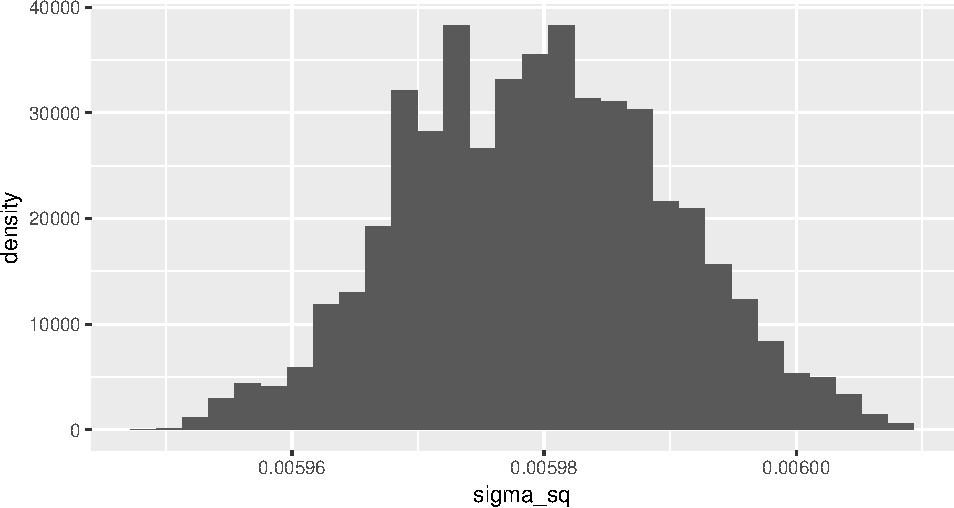
\includegraphics{20190225_bayes_MCMC_Metropolis_files/figure-latex/unnamed-chunk-10-1.pdf}

\begin{Shaded}
\begin{Highlighting}[]
\KeywordTok{ggplot}\NormalTok{() }\OperatorTok{+}
\StringTok{  }\KeywordTok{geom_density}\NormalTok{(}\DataTypeTok{data =}\NormalTok{ theta_posterior_sample, }\DataTypeTok{mapping =} \KeywordTok{aes}\NormalTok{(}\DataTypeTok{x =}\NormalTok{ sigma_sq))}
\end{Highlighting}
\end{Shaded}

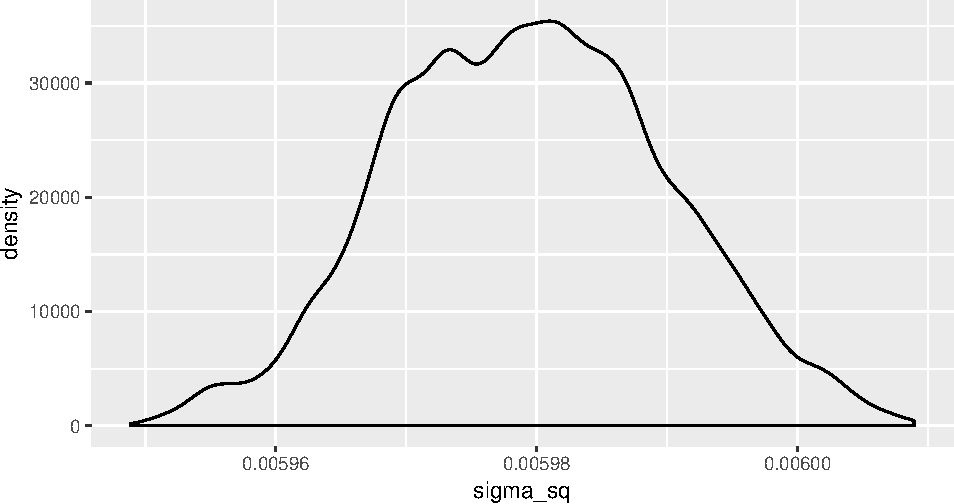
\includegraphics{20190225_bayes_MCMC_Metropolis_files/figure-latex/unnamed-chunk-11-1.pdf}

\newpage

\paragraph{How does the model fit?}\label{how-does-the-model-fit}

Compare a histogram of the data to the normal density with parameters
set equal to the estimated posterior mean for \(\mu\) and for
\(\sigma^2\).

\begin{Shaded}
\begin{Highlighting}[]
\KeywordTok{ggplot}\NormalTok{(}\DataTypeTok{data =}\NormalTok{ cmb, }\DataTypeTok{mapping =} \KeywordTok{aes}\NormalTok{(}\DataTypeTok{x =}\NormalTok{ temp_difference)) }\OperatorTok{+}
\StringTok{  }\KeywordTok{geom_histogram}\NormalTok{(}\DataTypeTok{center =} \FloatTok{0.005}\NormalTok{, }\DataTypeTok{binwidth =} \FloatTok{0.01}\NormalTok{, }\DataTypeTok{mapping =} \KeywordTok{aes}\NormalTok{(}\DataTypeTok{y =}\NormalTok{ ..density..)) }\OperatorTok{+}
\StringTok{  }\KeywordTok{stat_function}\NormalTok{(}\DataTypeTok{fun =}\NormalTok{ dnorm,}
    \DataTypeTok{args =} \KeywordTok{list}\NormalTok{(}\DataTypeTok{mean =} \KeywordTok{mean}\NormalTok{(theta_posterior_sample}\OperatorTok{$}\NormalTok{mu), }\DataTypeTok{sd =} \KeywordTok{sqrt}\NormalTok{(}\KeywordTok{mean}\NormalTok{(theta_posterior_sample}\OperatorTok{$}\NormalTok{sigma_sq))))}
\end{Highlighting}
\end{Shaded}

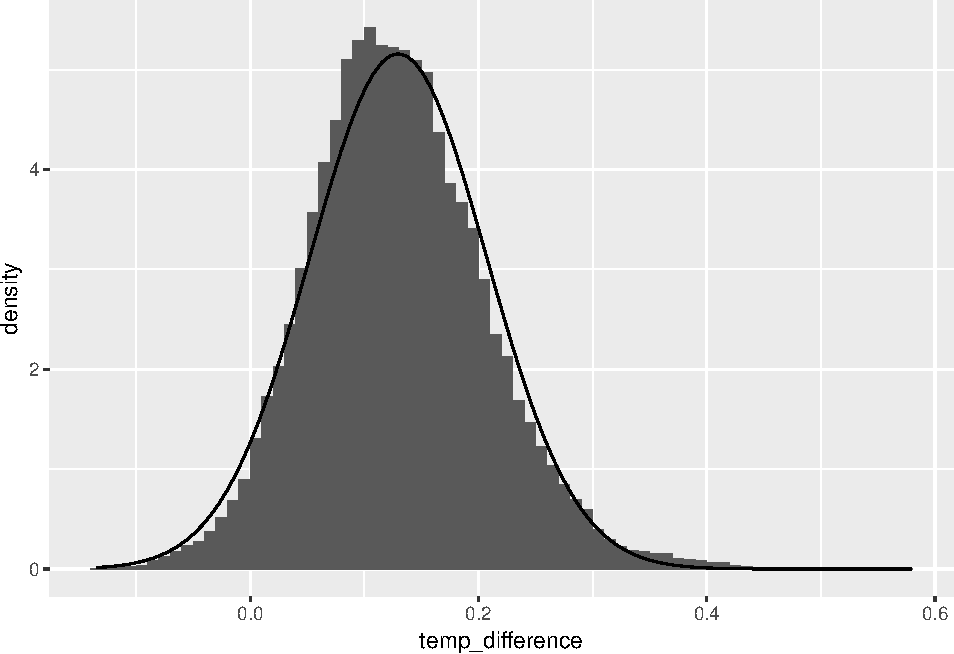
\includegraphics{20190225_bayes_MCMC_Metropolis_files/figure-latex/unnamed-chunk-12-1.pdf}

\subsection{Fit via Stan}\label{fit-via-stan}

\subsubsection{normal.stan}\label{normal.stan}

Here is the content of the file normal.stan:

\begin{Shaded}
\begin{Highlighting}[]
\NormalTok{data \{}
\NormalTok{  int}\OperatorTok{<}\NormalTok{lower=}\DecValTok{0}\OperatorTok{>}\StringTok{ }\NormalTok{n; }\OperatorTok{/}\ErrorTok{/}\StringTok{ }\NormalTok{number of observations}
\NormalTok{  real x[n]; }\OperatorTok{/}\ErrorTok{/}\StringTok{ }\NormalTok{data}\OperatorTok{:}\StringTok{ }\NormalTok{an array of length n where each entry is a real number}
\NormalTok{\}}

\NormalTok{parameters \{}
\NormalTok{  real mu;}
\NormalTok{  real}\OperatorTok{<}\NormalTok{lower=}\DecValTok{0}\OperatorTok{>}\StringTok{ }\NormalTok{sigma;}
\NormalTok{\}}

\NormalTok{model \{}
\NormalTok{  mu }\OperatorTok{~}\StringTok{ }\KeywordTok{normal}\NormalTok{(}\DecValTok{0}\NormalTok{, }\DecValTok{1000}\NormalTok{); }\OperatorTok{/}\ErrorTok{/}\StringTok{ }\NormalTok{prior }\ControlFlowTok{for}\NormalTok{ mu}\OperatorTok{:}\StringTok{ }\NormalTok{normal with a very large variance; non}\OperatorTok{-}\NormalTok{informative}
\NormalTok{  sigma }\OperatorTok{~}\StringTok{ }\KeywordTok{gamma}\NormalTok{(}\DecValTok{2}\NormalTok{, }\DecValTok{1}\NormalTok{); }\OperatorTok{/}\ErrorTok{/}\StringTok{ }\NormalTok{prior }\ControlFlowTok{for}\NormalTok{ sigma}\OperatorTok{:}\StringTok{ }\NormalTok{gamma with shape =}\StringTok{ }\DecValTok{1}\NormalTok{ and rate =}\StringTok{ }\FloatTok{0.01}\NormalTok{; non}\OperatorTok{-}\NormalTok{informative}
\NormalTok{  x }\OperatorTok{~}\StringTok{ }\KeywordTok{normal}\NormalTok{(mu, sigma); }\OperatorTok{/}\ErrorTok{/}\StringTok{ }\NormalTok{data model}\OperatorTok{:}\StringTok{ }\NormalTok{each element of x follows a }\KeywordTok{normal}\NormalTok{(mu, sigma) distribution}
\NormalTok{\}}
\end{Highlighting}
\end{Shaded}

The \texttt{data} block in the Stan file describes fixed, known
quantities that will be passed in to Stan. In this case, we have said
that we will tell Stan what our sample size is (\texttt{n}) and give it
a vector of length \texttt{n} with observed data values \texttt{x}.

The \texttt{parameters} block defines parameters to estimate; in this
case, the mean \texttt{mu} and standard deviation \texttt{sigma} of the
normal distribution.

The \texttt{model} block defines our prior distributions and data model.

Stan takes these ingredients and creates a program in C++ that will
perform Bayesian estimation for this model using a MCMC approach called
Hamiltonian Monte Carlo.

\subsubsection{R code to interface with
Stan}\label{r-code-to-interface-with-stan}

\paragraph{Call Stan to do the
estimation}\label{call-stan-to-do-the-estimation}

\begin{itemize}
\tightlist
\item
  For MCMC, just one command (\texttt{stan}) both compiles the model and
  performs the sampling.
\item
  A substantial part of the run time when calling Stan comes from
  creating and compiling the C++ program to do estimation. The command
  \texttt{rstan\_options(auto\_write\ =\ TRUE)} ensures that this is
  done only the first time you call Stan, unless you've made changes to
  the stan file.
\item
  The \texttt{stan} function does estimation. Here we have used 4
  arguments:

  \begin{itemize}
  \tightlist
  \item
    \texttt{file}: the stan file with the model definition, created
    above.
  \item
    \texttt{data}: a named list with one entry for each variable
    declared in the \texttt{data} block of the stan file.
  \item
    \texttt{iter}: how many iterations to perform (how many samples to
    draw from the posterior in each MCMC chain).
  \item
    \texttt{chains}: how many MCMC chains to run; here, 4 separate
    chains are run.
  \end{itemize}
\end{itemize}

\begin{Shaded}
\begin{Highlighting}[]
\KeywordTok{library}\NormalTok{(rstan)}
\end{Highlighting}
\end{Shaded}

\begin{verbatim}
## Warning: package 'StanHeaders' was built under R version 3.5.2
\end{verbatim}

\begin{Shaded}
\begin{Highlighting}[]
\KeywordTok{rstan_options}\NormalTok{(}\DataTypeTok{auto_write =} \OtherTok{TRUE}\NormalTok{)}

\NormalTok{fit <-}\StringTok{ }\KeywordTok{stan}\NormalTok{(}
  \DataTypeTok{file =} \StringTok{"normal.stan"}\NormalTok{,}
  \DataTypeTok{data =} \KeywordTok{list}\NormalTok{(}\DataTypeTok{n =} \KeywordTok{nrow}\NormalTok{(cmb), }\DataTypeTok{x =}\NormalTok{ cmb}\OperatorTok{$}\NormalTok{temp_difference),}
  \DataTypeTok{iter =} \DecValTok{1000}\NormalTok{,}
  \DataTypeTok{chains =} \DecValTok{4}\NormalTok{)}
\end{Highlighting}
\end{Shaded}

\begin{verbatim}
## 
## SAMPLING FOR MODEL 'normal' NOW (CHAIN 1).
## Chain 1: 
## Chain 1: Gradient evaluation took 0.002114 seconds
## Chain 1: 1000 transitions using 10 leapfrog steps per transition would take 21.14 seconds.
## Chain 1: Adjust your expectations accordingly!
## Chain 1: 
## Chain 1: 
## Chain 1: Iteration:   1 / 1000 [  0%]  (Warmup)
## Chain 1: Iteration: 100 / 1000 [ 10%]  (Warmup)
## Chain 1: Iteration: 200 / 1000 [ 20%]  (Warmup)
## Chain 1: Iteration: 300 / 1000 [ 30%]  (Warmup)
## Chain 1: Iteration: 400 / 1000 [ 40%]  (Warmup)
## Chain 1: Iteration: 500 / 1000 [ 50%]  (Warmup)
## Chain 1: Iteration: 501 / 1000 [ 50%]  (Sampling)
## Chain 1: Iteration: 600 / 1000 [ 60%]  (Sampling)
## Chain 1: Iteration: 700 / 1000 [ 70%]  (Sampling)
## Chain 1: Iteration: 800 / 1000 [ 80%]  (Sampling)
## Chain 1: Iteration: 900 / 1000 [ 90%]  (Sampling)
## Chain 1: Iteration: 1000 / 1000 [100%]  (Sampling)
## Chain 1: 
## Chain 1:  Elapsed Time: 13.4016 seconds (Warm-up)
## Chain 1:                15.1235 seconds (Sampling)
## Chain 1:                28.5251 seconds (Total)
## Chain 1: 
## 
## SAMPLING FOR MODEL 'normal' NOW (CHAIN 2).
## Chain 2: 
## Chain 2: Gradient evaluation took 0.002252 seconds
## Chain 2: 1000 transitions using 10 leapfrog steps per transition would take 22.52 seconds.
## Chain 2: Adjust your expectations accordingly!
## Chain 2: 
## Chain 2: 
## Chain 2: Iteration:   1 / 1000 [  0%]  (Warmup)
## Chain 2: Iteration: 100 / 1000 [ 10%]  (Warmup)
## Chain 2: Iteration: 200 / 1000 [ 20%]  (Warmup)
## Chain 2: Iteration: 300 / 1000 [ 30%]  (Warmup)
## Chain 2: Iteration: 400 / 1000 [ 40%]  (Warmup)
## Chain 2: Iteration: 500 / 1000 [ 50%]  (Warmup)
## Chain 2: Iteration: 501 / 1000 [ 50%]  (Sampling)
## Chain 2: Iteration: 600 / 1000 [ 60%]  (Sampling)
## Chain 2: Iteration: 700 / 1000 [ 70%]  (Sampling)
## Chain 2: Iteration: 800 / 1000 [ 80%]  (Sampling)
## Chain 2: Iteration: 900 / 1000 [ 90%]  (Sampling)
## Chain 2: Iteration: 1000 / 1000 [100%]  (Sampling)
## Chain 2: 
## Chain 2:  Elapsed Time: 7.18012 seconds (Warm-up)
## Chain 2:                15.2367 seconds (Sampling)
## Chain 2:                22.4168 seconds (Total)
## Chain 2: 
## 
## SAMPLING FOR MODEL 'normal' NOW (CHAIN 3).
## Chain 3: 
## Chain 3: Gradient evaluation took 0.00231 seconds
## Chain 3: 1000 transitions using 10 leapfrog steps per transition would take 23.1 seconds.
## Chain 3: Adjust your expectations accordingly!
## Chain 3: 
## Chain 3: 
## Chain 3: Iteration:   1 / 1000 [  0%]  (Warmup)
## Chain 3: Iteration: 100 / 1000 [ 10%]  (Warmup)
## Chain 3: Iteration: 200 / 1000 [ 20%]  (Warmup)
## Chain 3: Iteration: 300 / 1000 [ 30%]  (Warmup)
## Chain 3: Iteration: 400 / 1000 [ 40%]  (Warmup)
## Chain 3: Iteration: 500 / 1000 [ 50%]  (Warmup)
## Chain 3: Iteration: 501 / 1000 [ 50%]  (Sampling)
## Chain 3: Iteration: 600 / 1000 [ 60%]  (Sampling)
## Chain 3: Iteration: 700 / 1000 [ 70%]  (Sampling)
## Chain 3: Iteration: 800 / 1000 [ 80%]  (Sampling)
## Chain 3: Iteration: 900 / 1000 [ 90%]  (Sampling)
## Chain 3: Iteration: 1000 / 1000 [100%]  (Sampling)
## Chain 3: 
## Chain 3:  Elapsed Time: 15.9207 seconds (Warm-up)
## Chain 3:                15.3833 seconds (Sampling)
## Chain 3:                31.304 seconds (Total)
## Chain 3: 
## 
## SAMPLING FOR MODEL 'normal' NOW (CHAIN 4).
## Chain 4: 
## Chain 4: Gradient evaluation took 0.002014 seconds
## Chain 4: 1000 transitions using 10 leapfrog steps per transition would take 20.14 seconds.
## Chain 4: Adjust your expectations accordingly!
## Chain 4: 
## Chain 4: 
## Chain 4: Iteration:   1 / 1000 [  0%]  (Warmup)
## Chain 4: Iteration: 100 / 1000 [ 10%]  (Warmup)
## Chain 4: Iteration: 200 / 1000 [ 20%]  (Warmup)
## Chain 4: Iteration: 300 / 1000 [ 30%]  (Warmup)
## Chain 4: Iteration: 400 / 1000 [ 40%]  (Warmup)
## Chain 4: Iteration: 500 / 1000 [ 50%]  (Warmup)
## Chain 4: Iteration: 501 / 1000 [ 50%]  (Sampling)
## Chain 4: Iteration: 600 / 1000 [ 60%]  (Sampling)
## Chain 4: Iteration: 700 / 1000 [ 70%]  (Sampling)
## Chain 4: Iteration: 800 / 1000 [ 80%]  (Sampling)
## Chain 4: Iteration: 900 / 1000 [ 90%]  (Sampling)
## Chain 4: Iteration: 1000 / 1000 [100%]  (Sampling)
## Chain 4: 
## Chain 4:  Elapsed Time: 19.4481 seconds (Warm-up)
## Chain 4:                13.0007 seconds (Sampling)
## Chain 4:                32.4487 seconds (Total)
## Chain 4:
\end{verbatim}

\paragraph{View the results}\label{view-the-results}

The \texttt{rstan} package comes with some pretty useful default
functions to display and summarize the samples from the posterior
distribution:

\begin{Shaded}
\begin{Highlighting}[]
\KeywordTok{print}\NormalTok{(fit)}
\end{Highlighting}
\end{Shaded}

\begin{verbatim}
## Inference for Stan model: normal.
## 4 chains, each with iter=1000; warmup=500; thin=1; 
## post-warmup draws per chain=500, total post-warmup draws=2000.
## 
##             mean se_mean   sd       2.5%        25%        50%        75%
## mu          0.13    0.00 0.00       0.13       0.13       0.13       0.13
## sigma       0.08    0.00 0.00       0.08       0.08       0.08       0.08
## lp__  1318253.74    0.04 0.96 1318251.10 1318253.38 1318254.02 1318254.42
##            97.5% n_eff Rhat
## mu          0.13  1977 1.00
## sigma       0.08   296 1.02
## lp__  1318254.68   576 1.01
## 
## Samples were drawn using NUTS(diag_e) at Thu Feb 28 21:48:54 2019.
## For each parameter, n_eff is a crude measure of effective sample size,
## and Rhat is the potential scale reduction factor on split chains (at 
## convergence, Rhat=1).
\end{verbatim}

\begin{Shaded}
\begin{Highlighting}[]
\KeywordTok{plot}\NormalTok{(fit)}
\end{Highlighting}
\end{Shaded}

\begin{verbatim}
## ci_level: 0.8 (80% intervals)
\end{verbatim}

\begin{verbatim}
## outer_level: 0.95 (95% intervals)
\end{verbatim}

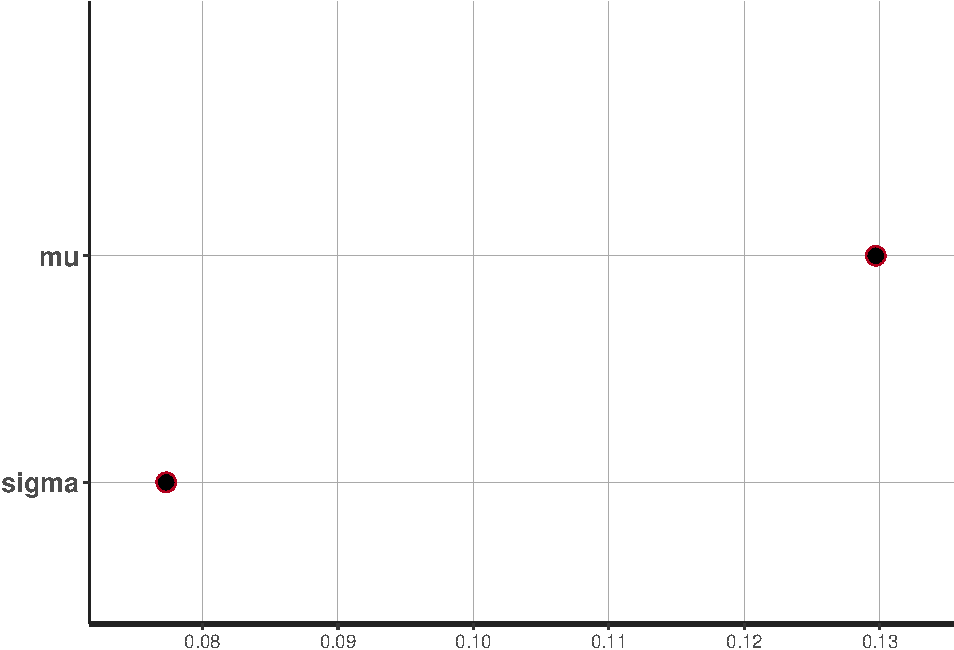
\includegraphics{20190225_bayes_MCMC_Metropolis_files/figure-latex/unnamed-chunk-15-1.pdf}

\begin{Shaded}
\begin{Highlighting}[]
\KeywordTok{pairs}\NormalTok{(fit, }\DataTypeTok{pars =} \KeywordTok{c}\NormalTok{(}\StringTok{"mu"}\NormalTok{, }\StringTok{"sigma"}\NormalTok{))}
\end{Highlighting}
\end{Shaded}

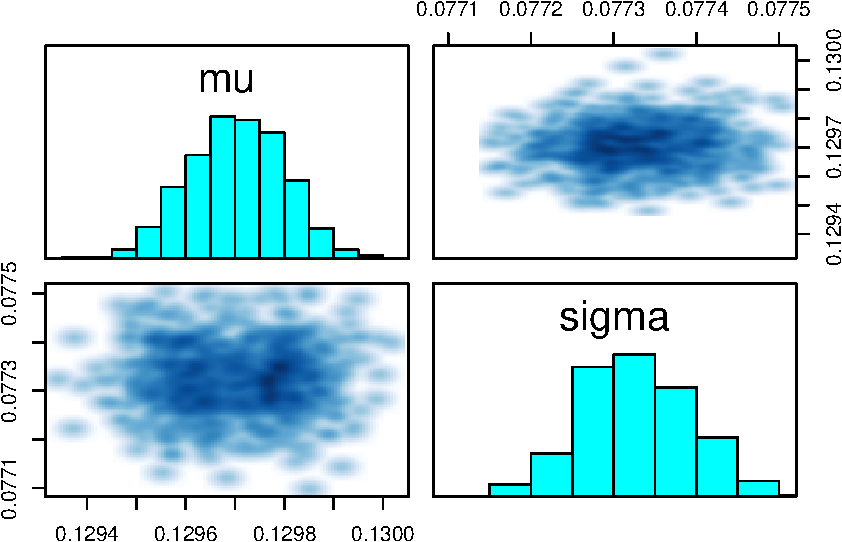
\includegraphics{20190225_bayes_MCMC_Metropolis_files/figure-latex/unnamed-chunk-15-2.pdf}

We can also extract the parameter samples and compute summaries like
posterior means and credible intervals by hand. Calling
\texttt{as.data.frame} on our model fit object returns a data frame with
the samples for each parameter defined in the stan model file.

\begin{Shaded}
\begin{Highlighting}[]
\NormalTok{param_samples <-}\StringTok{ }\KeywordTok{as.data.frame}\NormalTok{(fit)}

\KeywordTok{head}\NormalTok{(param_samples)}
\end{Highlighting}
\end{Shaded}

\begin{verbatim}
##          mu      sigma    lp__
## 1 0.1297261 0.07732078 1318255
## 2 0.1297270 0.07742988 1318253
## 3 0.1297446 0.07732818 1318255
## 4 0.1297443 0.07741279 1318254
## 5 0.1297420 0.07735710 1318254
## 6 0.1296313 0.07734655 1318254
\end{verbatim}

\begin{Shaded}
\begin{Highlighting}[]
\KeywordTok{dim}\NormalTok{(param_samples)}
\end{Highlighting}
\end{Shaded}

\begin{verbatim}
## [1] 2000    3
\end{verbatim}

\begin{Shaded}
\begin{Highlighting}[]
\NormalTok{param_samples }\OperatorTok
\StringTok{  }\KeywordTok{summarize}\NormalTok{(}
    \DataTypeTok{mu_mean =} \KeywordTok{mean}\NormalTok{(mu),}
    \DataTypeTok{mu_ci_lower =} \KeywordTok{quantile}\NormalTok{(mu, }\DataTypeTok{probs =} \FloatTok{0.025}\NormalTok{),}
    \DataTypeTok{mu_ci_upper =} \KeywordTok{quantile}\NormalTok{(mu, }\DataTypeTok{probs =} \FloatTok{0.975}\NormalTok{),}
    \DataTypeTok{sigma_mean =} \KeywordTok{mean}\NormalTok{(sigma),}
    \DataTypeTok{sigma_ci_lower =} \KeywordTok{quantile}\NormalTok{(sigma, }\DataTypeTok{probs =} \FloatTok{0.025}\NormalTok{),}
    \DataTypeTok{sigma_ci_upper =} \KeywordTok{quantile}\NormalTok{(sigma, }\DataTypeTok{probs =} \FloatTok{0.975}\NormalTok{)}
\NormalTok{  )}
\end{Highlighting}
\end{Shaded}

\begin{verbatim}
##     mu_mean mu_ci_lower mu_ci_upper sigma_mean sigma_ci_lower
## 1 0.1297032    0.129516   0.1298862 0.07732648     0.07719778
##   sigma_ci_upper
## 1     0.07745808
\end{verbatim}

\begin{Shaded}
\begin{Highlighting}[]
\KeywordTok{ggplot}\NormalTok{(}\DataTypeTok{data =}\NormalTok{ param_samples, }\DataTypeTok{mapping =} \KeywordTok{aes}\NormalTok{(}\DataTypeTok{x =}\NormalTok{ mu)) }\OperatorTok{+}
\StringTok{  }\KeywordTok{geom_density}\NormalTok{()}
\end{Highlighting}
\end{Shaded}

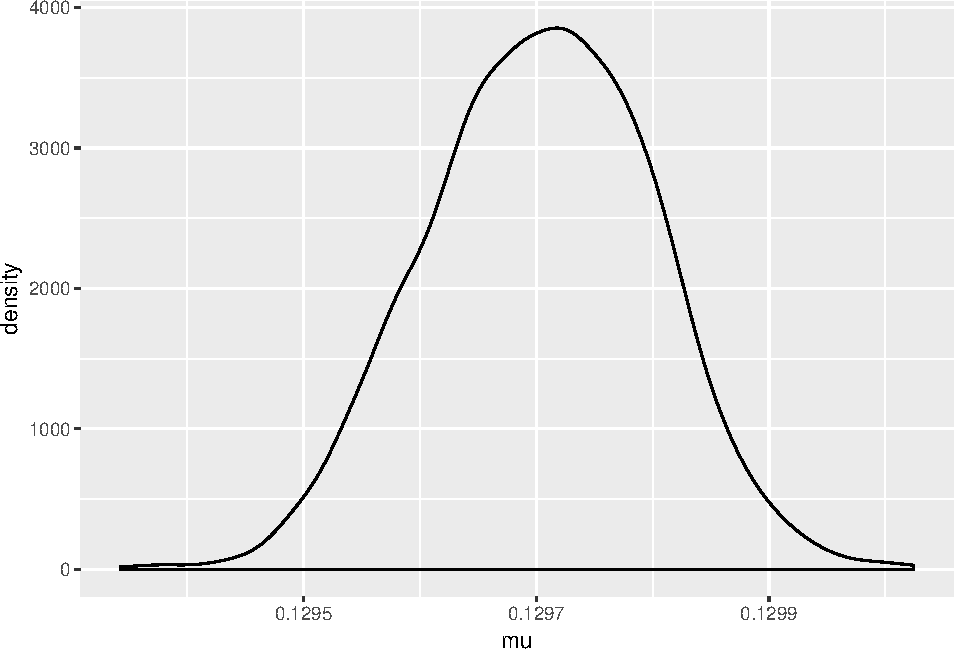
\includegraphics{20190225_bayes_MCMC_Metropolis_files/figure-latex/unnamed-chunk-17-1.pdf}


\end{document}
